\subsection{Méthode des moments}

a) Nous avons généré à l’aide de la fonction \texttt{wblrnd} de Matlab un échantillon de taille 1000 avec $\theta = (k,c) = (3.7,4.2)$. Nous avons tracé l'histogramme de l’échantillon obtenu (voir figure~\ref{fig:histo1}) et avons trouvé que 
\begin{align*}
\overline{x} &= \frac{1}{n}\sum\limits_{i=1}^n x_i &= 3.8036\\
s^2 &= \frac{1}{n-1}\sum\limits_{i=1}^n(x_i-\overline{x}) &= 1.3549\\
cv &= \frac{s}{\overline{x}} &= 0.3060
\end{align*}

\begin{figure}[!ht]
        \centering
        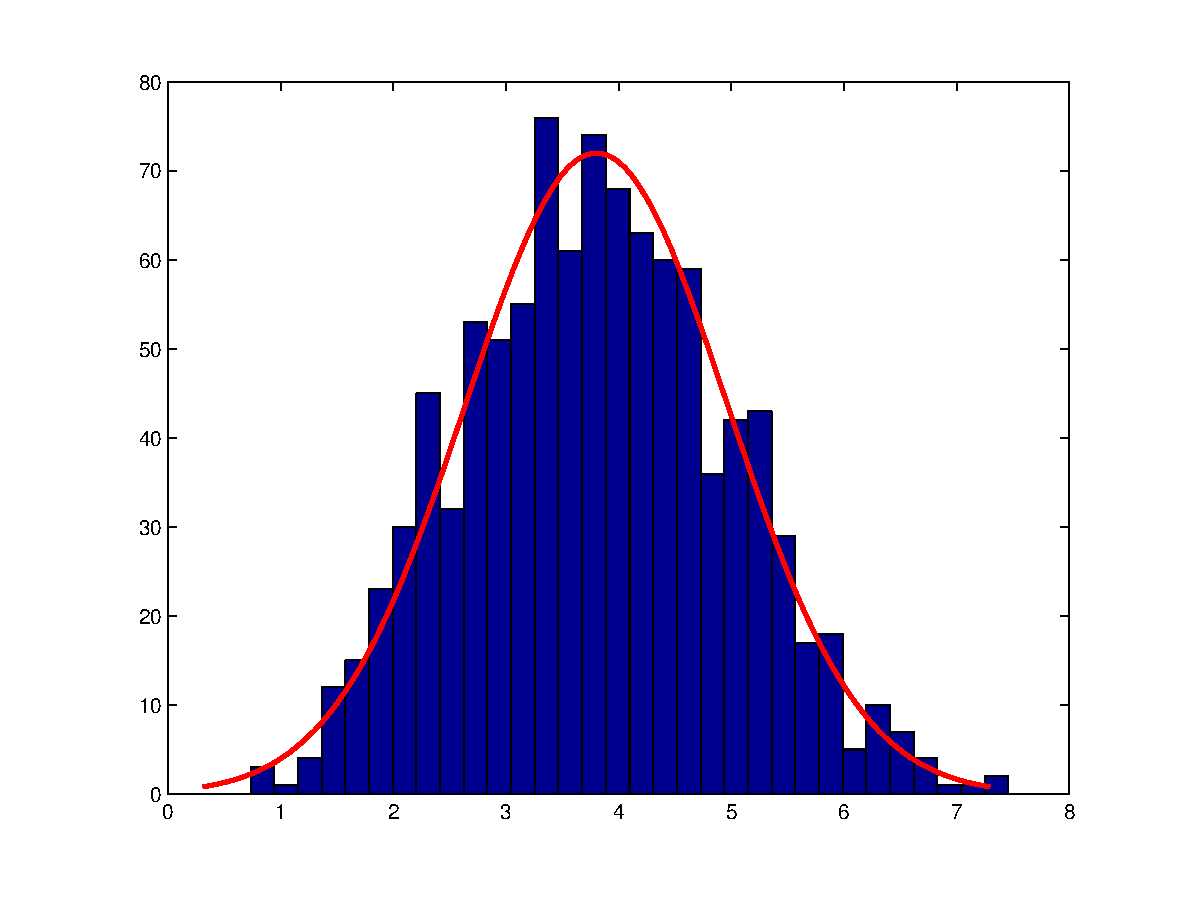
\includegraphics[width=0.4\textwidth]{graphes/histo1.eps}
        \caption{Histogramme pour un échantillon de taille 1000 avec k = 3.7 et c = 4.2}\label{fig:histo1}
\end{figure}

b)  Utilisons maintenant la méthode des moments pour trouver un estimateur $\hat\theta_{MM}$. Nous avons
\begin{align*}
\mu_1 = \mathbb{E}(x) &= \int_0^\infty \! x \frac{k}{c} \left(\frac{x}{c}\right)^{k-1} exp\left(-\left(\frac{x}{c}\right)^k\right) \, \mathrm{d}x
= \int_0^\infty \! c y^{\frac{1}{k}} exp(-y) \, \mathrm{d}y
= c\Gamma\left(\frac{1}{k}+1\right)
\end{align*}
\begin{align*}
\mu_2 = \mathbb{E}(x^2) &= \int_0^\infty \! x^2 \frac{k}{c} \left(\frac{x}{c}\right)^{k-1} exp\left(-\left(\frac{x}{c}\right)^k\right) \, \mathrm{d}x
= \int_0^\infty \! c^2 y^{\frac{2}{k}} exp(-y) \, \mathrm{d}y
= c^2\Gamma\left(\frac{2}{k}+1\right)
\end{align*}

La méthode des moments consiste à résoudre
\[
\left\{
\begin{array}{r c l}
\overline{x}  &=& c\Gamma\left(\frac{1}{k}+1\right)\\
\frac{1}{n}\sum\limits_{i=1}^n x_i ^2 &=& c^2\Gamma\left(\frac{2}{k}+1\right)
\end{array}
\right.
\]
où k et c trouvés seront $\hat{k}_{MM}$ et $\hat{c}_{MM}$.\\

c) On trouve $\hat{k}_{MM}$ en résolvant 
$$ \frac{1}{n}\sum\limits_{i=1}^n x_i ^2 = 15.8212 = \left(\frac{3.8036}{\Gamma\left(\frac{1}{k}+1\right)}\right)^2\Gamma\left(\frac{2}{k}+1\right)$$
à l'aide de la méthode de la bissection et $\hat{c}_{MM}$ en réinjectant ce résultat dans la première équation de notre système. On trouve $\hat{\theta} = (3.6343,4.2189)$ et donc $ERT = (\hat{k}_{MM} - k)^2 +(\hat{c}_{MM} - c)^2 = 0.0047$. \\

d) Nous avons effectué 500 réplications en calculant $\hat{\theta}_{MM}$ et ERT pour chaque réplication. Voici la moyenne et la variance de ces séries.
\begin{center}
\begin{tabular}{|c|c|c|c|}
  \hline
   &  $\hat{k}_{MM}$ & $\hat{c}_{MM}$ & ERT \\
  \hline
  Moyenne & 3.7025 & 4.1976 & 0.0098 \\
  Variance & 0.0085 & 0.0014 & 0.0001 \\
  \hline
\end{tabular}
\end{center}

e) Pour chaque série, nous avons produit un box-plot et un histogramme. Les graphes relatifs à $\hat{k}$ se retrouvent à la figure~\ref{fig:kmm}, ceux de $\hat{c}$ à la figure~\ref{fig:cmm} et ceux de $ERT$ à la figure~\ref{fig:ertmm}.\\

\begin{figure}[!ht]
        \centering
        \begin{subfigure}[b]{0.4\textwidth}
                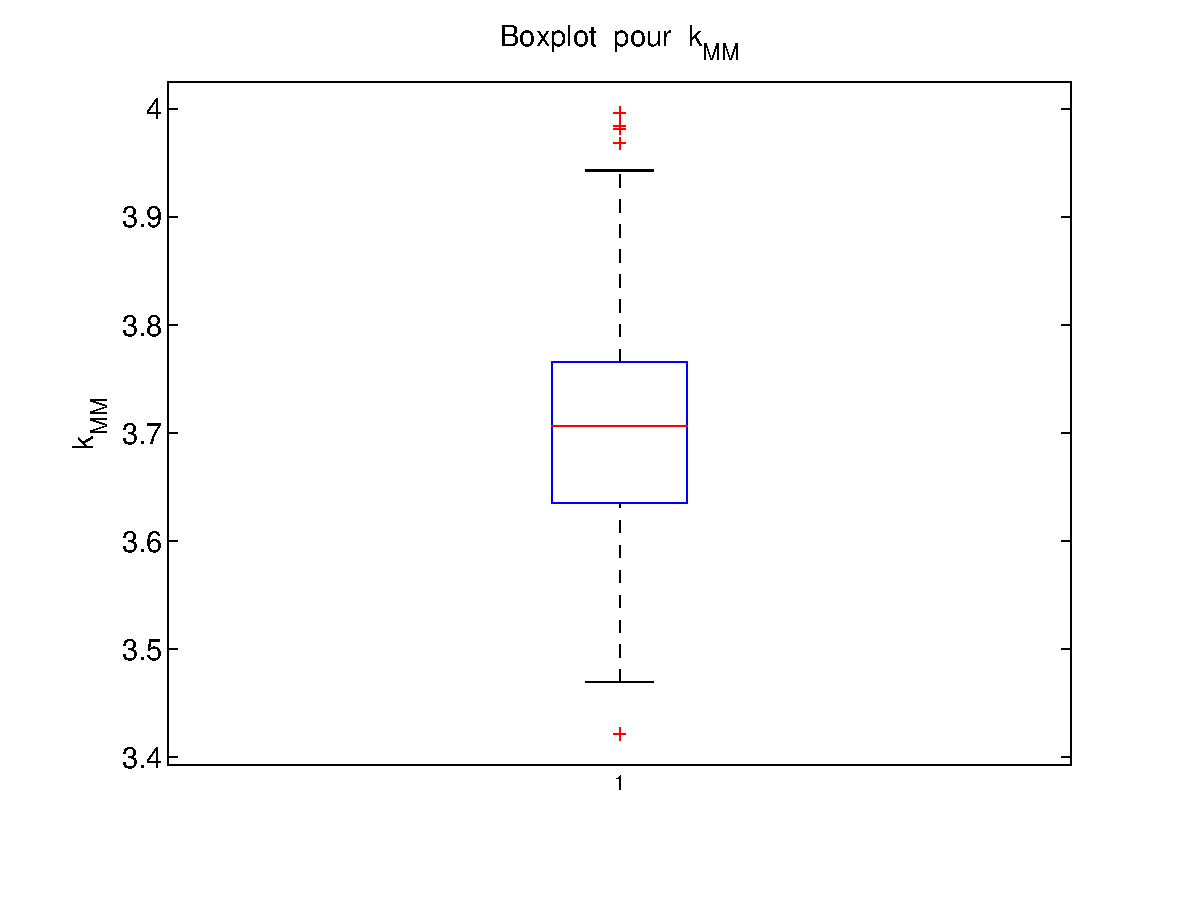
\includegraphics[width=\textwidth]{graphes/boxplot_kmm.eps}
        \end{subfigure}%
        ~
        \begin{subfigure}[b]{0.4\textwidth}
                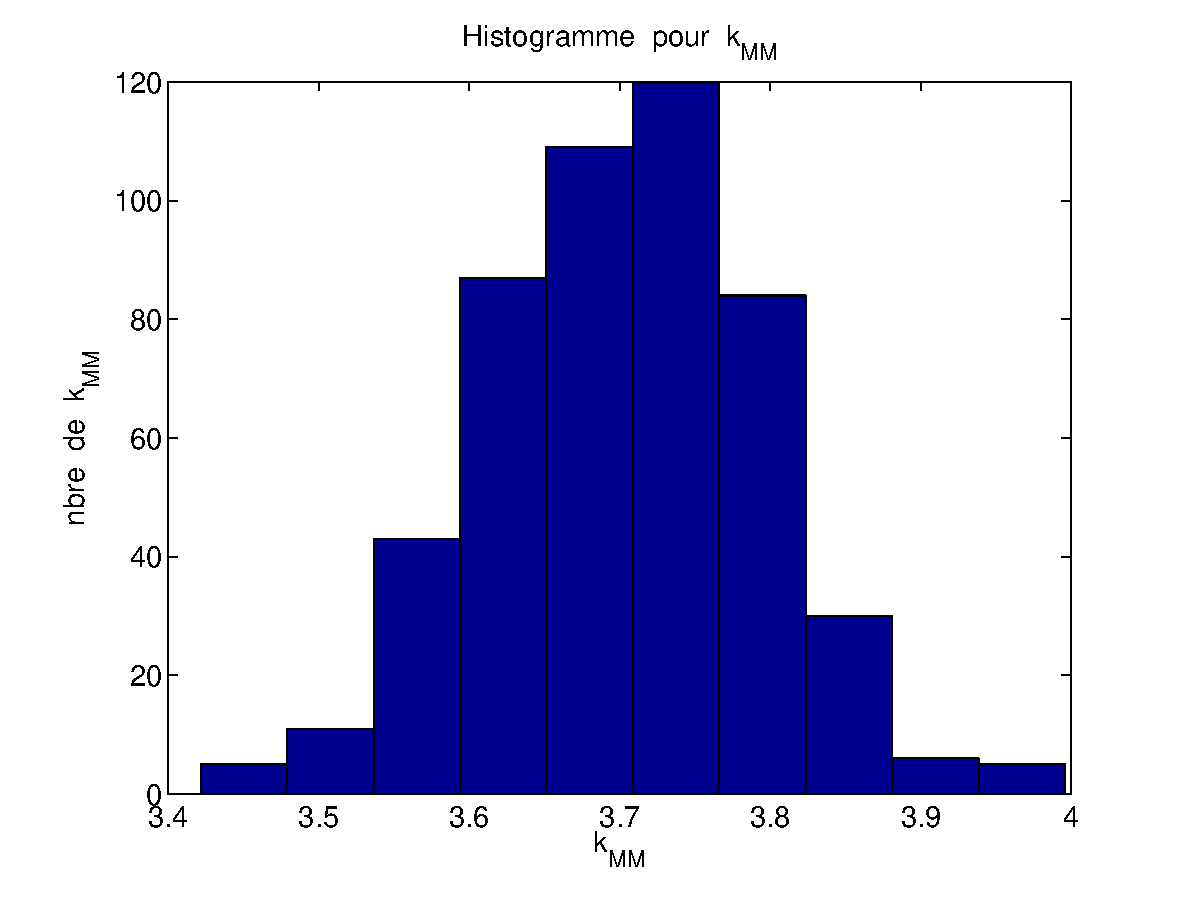
\includegraphics[width=\textwidth]{graphes/hist_kmm.eps}
        \end{subfigure}
        \caption{Graphes pour $\hat{k}$}\label{fig:kmm}
\end{figure}

\begin{figure}[!ht]
        \centering
        \begin{subfigure}[b]{0.4\textwidth}
                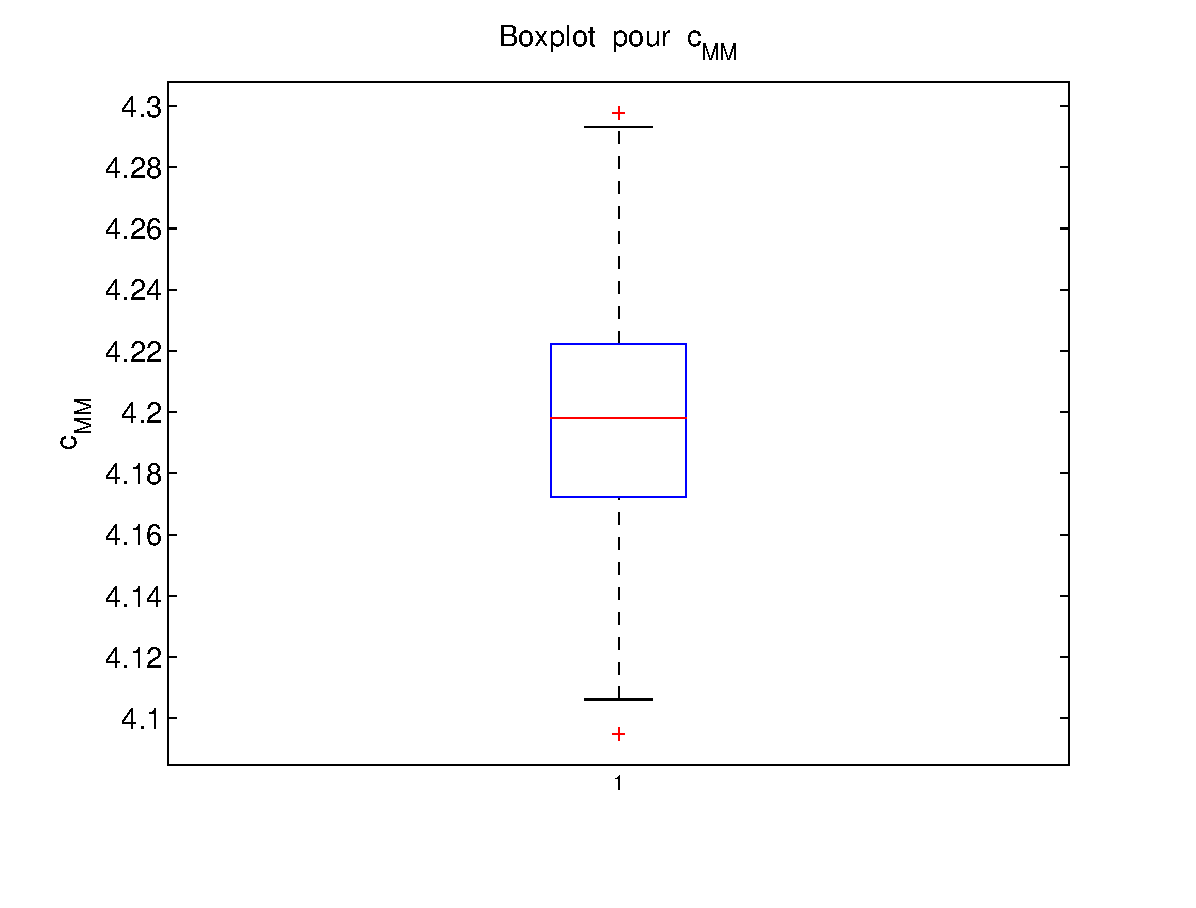
\includegraphics[width=\textwidth]{graphes/boxplot_cmm.eps}
        \end{subfigure}%
        ~
        \begin{subfigure}[b]{0.4\textwidth}
                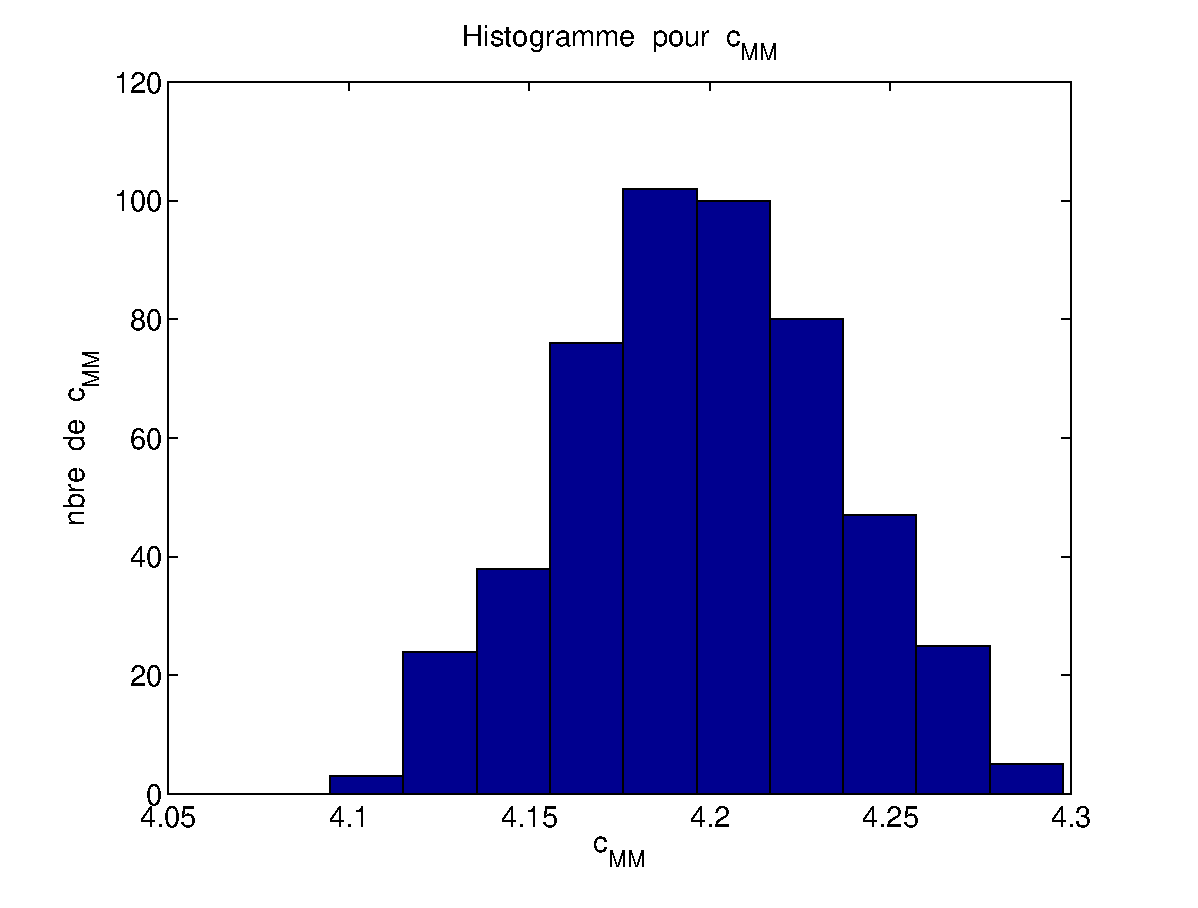
\includegraphics[width=\textwidth]{graphes/hist_cmm.eps}
        \end{subfigure}
        \caption{Graphes pour $\hat{c}$}\label{fig:cmm}
\end{figure}

\begin{figure}[!ht]
        \centering
        \begin{subfigure}[b]{0.4\textwidth}
                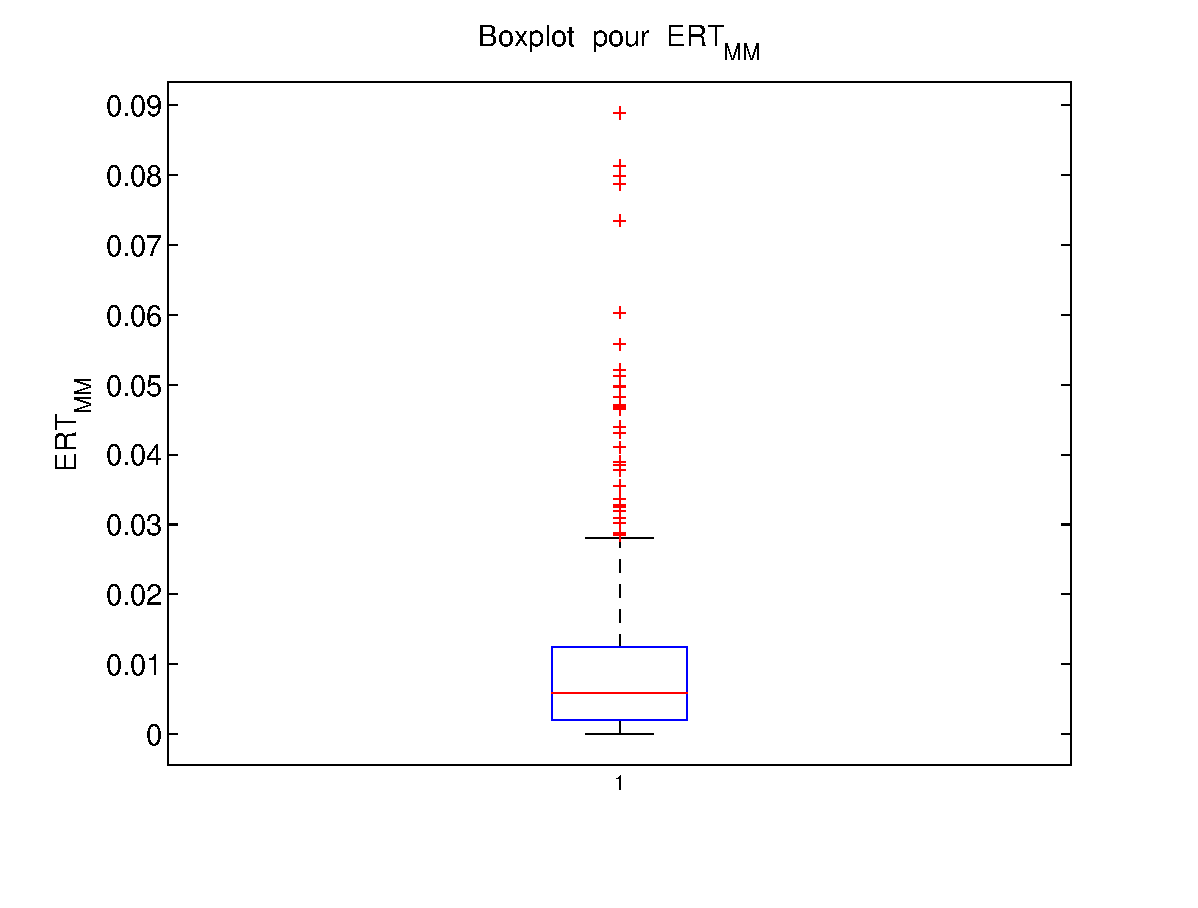
\includegraphics[width=\textwidth]{graphes/boxplot_ertmm.eps}
        \end{subfigure}%
        ~ 
        \begin{subfigure}[b]{0.4\textwidth}
                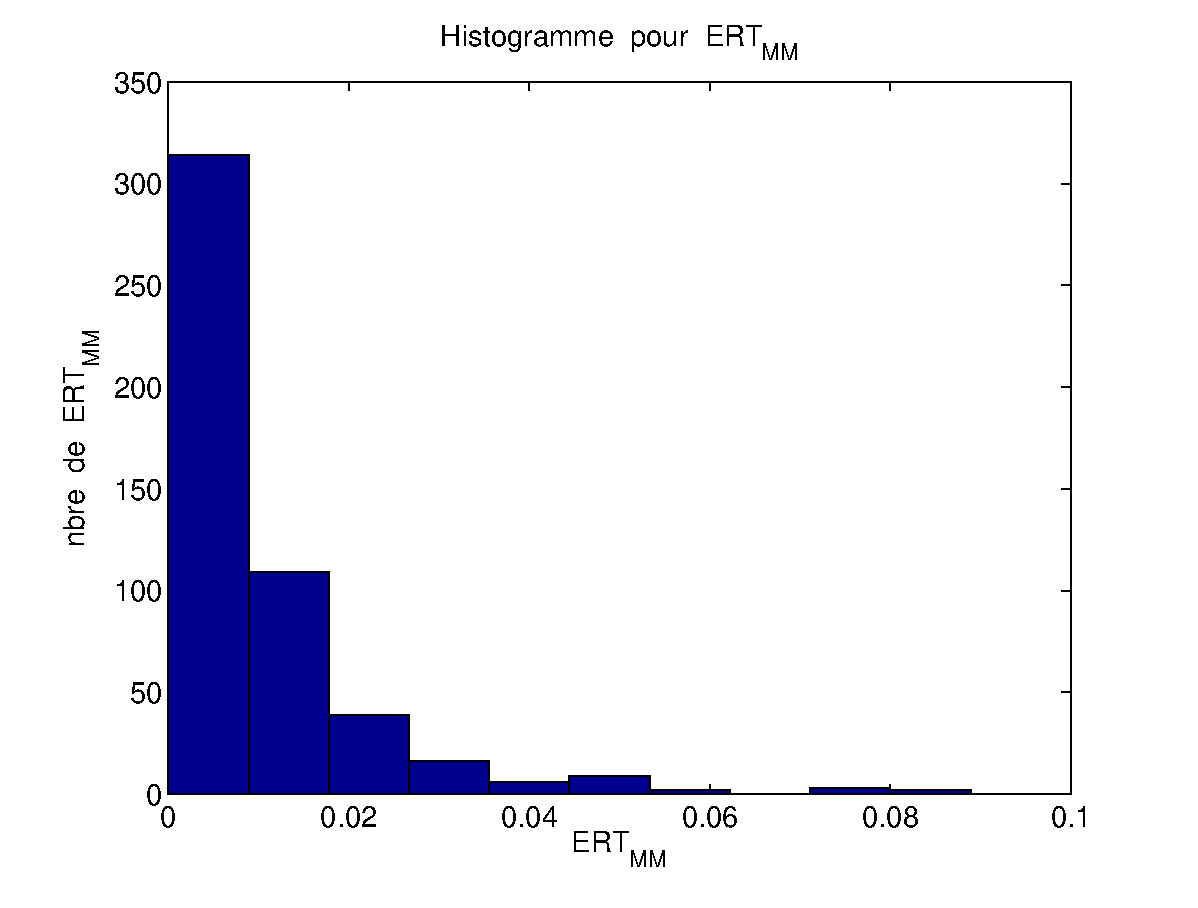
\includegraphics[width=\textwidth]{graphes/hist_ertmm.eps}
        \end{subfigure}
        \caption{Graphes pour $ERT$}\label{fig:ertmm}
\end{figure}

f) Le biais de notre estimateur $\hat\theta_{MM}$ est négligeable et il diminue lorsque $n$ augmente; on peut donc dire que cet estimateur est asymptotiquement non-biaisé. La variance est très petite et en prenant des échantillons de plus en plus grands, on observe qu'elle devient de plus en plus petite. $\hat\theta_{MM}$ est donc consistant. En ce qui concerne les distributions asymptotiques, les histogrammes montrent qu’elles sont approximativement normales.